\documentclass{article}
\usepackage{subcaption}
\usepackage{amsmath}
\usepackage{mathtools}
\usepackage{hyperref}
\usepackage{polski}
\usepackage[utf8]{inputenc}
\usepackage{titlesec}
\usepackage{scalerel}
\usepackage{upquote}
\usepackage{multicol}
\usepackage{graphicx}
\usepackage{tabularx}
\usepackage{blindtext}
\usepackage{color}
\usepackage{colortbl}
\usepackage{amsmath}
\usepackage{algorithm}
\usepackage[noend]{algpseudocode}
\usepackage{multicol}
\usepackage{braket}
\usepackage[dvipdfmx]{media9}
\definecolor{dkgreen}{rgb}{0,0.6,0}
\definecolor{gray}{rgb}{0.5,0.5,0.5}
\definecolor{mauve}{rgb}{0.58,0,0.82}
\usepackage{geometry}
 \geometry{
 a4paper,
 total={170mm,257mm},
 left=20mm,
 top=20mm,
 }
\usepackage{placeins}
\usepackage{svg}
\newcolumntype{s}{>{\columncolor{yellow}}c}
\newcolumntype{h}{>{\columncolor{pink}}c}
\usepackage{listings}
\usepackage{float}

\lstset{frame=tb,
  language=Matlab,
  aboveskip=3mm,
  belowskip=3mm,
  showstringspaces=false,
  columns=flexible,
  basicstyle={\small\ttfamily},
  numbers=none,
  numberstyle=\tiny\color{gray},
  keywordstyle=\color{blue},
  commentstyle=\color{dkgreen},
  stringstyle=\color{mauve},
  breaklines=true,
  breakatwhitespace=true,
  tabsize=3
}
\usepackage[utf8]{inputenc}
\titleclass{\subsubsubsection}{straight}[\subsection]

\newcounter{subsubsubsection}[subsubsection]
\renewcommand\thesubsubsubsection{\thesubsubsection.\arabic{subsubsubsection}}

\titleformat{\subsubsubsection}
  {\normalfont\normalsize\bfseries}{\thesubsubsubsection}{1em}{}
\titlespacing*{\subsubsubsection}
{0pt}{3.25ex plus 1ex minus .2ex}{1.5ex plus .2ex}
\makeatletter
\def\toclevel@subsubsubsection{4}
\def\l@subsubsubsection{\@dottedtocline{4}{7em}{4em}}
\makeatother
\setcounter{secnumdepth}{4}
\setcounter{tocdepth}{4}


\title{Podstawy Obliczeń Komputerowych\\ Laboratorium 1}
\author{Kamil Czop 259613 \\ Łukasz Majchrzak 262761 \\ Wtorek 11:15TN - Y02-37c}
\date{28 marca 2023}

\begin{document}

\maketitle
\section{Metody obliczania równań liniowych}
\subsection{Cel ćwiczeń}
Celem przeprowadzonych laboratoriów było utworzenie programu rozwiązującego układ równań liniowych z wykorzystaniem dowolnej metody skończonej i iteracyjną.
\subsection{Dane}
\begin{figure}[H]
    \begin{multicols}{3}
        \begin{equation*}
         \mathbf{A}=\begin{bmatrix}2 & 1 & 1 & -1\\1 & 1 & -1 & 1\\ 1 & 1 & 1 & 1 \\ -1 & 2 & -1 & 1 \\\end{bmatrix}
        \end{equation*}
    \par
        \begin{equation*}
         \mathbf{B}=\begin{bmatrix}3 \\ 4 \\ 10 \\ 4\\\end{bmatrix}
        \end{equation*}
    \par
        \begin{equation*}
         \mathbf{AB}=\begin{bmatrix}2 & 1 & 1 & -1 & 3\\1 & 1 & 1 & -1 & 4\\ -1 & 2 & -1 & 1 & 10\\ -1 & 2 & -1 & 1 & 4\\\end{bmatrix}
        \end{equation*}
    \end{multicols}
\end{figure}

\subsection{Wykonanie} 
\subsection{Twierdzenie Kroneckera-Capellego}
Bazując na wymaganiach określonych w instrukcji laboratoryjnej wykonano początkowo program określającego z tw. Kroneckera-Capellego do wyznaczenia liczby rozwiązań naszego układu równań.
Po przepuszczeniu przez algorytm obliczający rangę macierzy w C++ i gotowej funkcji Matlab rank, dla macierzy $\mathbf{A}$ uzyskano wartość 4, a dla $
\mathbf{AB}$ także 4. Z tego wynika iż nasz układ równań posiadając równe rangi może posiadać jedno rozwiązanie układu. Posiadając potwierdzenie istnienia rozwiązania możemy rozwiązać układ metodą Gauss'a-Jordana.\\
\subsection{Metoda Gauss'a - Jordana}
\begin{algorithm}[H]
    \caption{Algorytm postępowania dla metody Gauss'a-Jordana}\label{euclid}
    \begin{algorithmic}[1]
        \Procedure{gaussJordan}{}
        \For {$i = 1 to n$}
            \If {$A_{i,i} = 0$}
                \State \textbf{Stop}
            \EndIf
            \For {$j = 1 to n$}
                \If{ $i != j$ }
                    \State $Ratio \gets A_{j,i} / A{i,i}$
                    \For {$k = 1 to n$}
                        \State {$A_{j,k} \gets A_{j,k} - Ratio * A{i,k}$}
                    \State \textbf{Next} $k$
                    \EndFor
                \EndIf
            \State \textbf{Next} $j$
            \EndFor
        \State \textbf{Next} $i$
        \EndFor
        \State \textbf{Stop}
        \EndProcedure
    \end{algorithmic}
\end{algorithm}
Metoda ta stanowi modyfikacje metody Gauss'a gdzie układ  równań liniowych jest sprowadzany do macierzy jednostkowej. W początkowej faczie poszerzamy macierz $\mathbf{A}$ o macierz $\mathbf{B}$ uzyskując macierz $\mathbf{AB}$. Macierz $AB$ przechodzi podaną transformacje. \\
\[
\begin{bmatrix} 
    A_{11} & \dots & A_{1n} & B_{1} \\
    \vdots & \ddots & \vdots & \vdots \\
    a_{n1} &  \dots & A_{nn}     & B_{n} 
    \end{bmatrix}
\qquad
\rightarrow \begin{bmatrix} 
    1 & \dots & 0 & B_{1}^{(n)} \\
    \vdots & \ddots & \vdots & \vdots \\
    0 &  \dots & 1    & B_{n}^{(n)} 
    \end{bmatrix}
\]\\
Wynikiem operacji na wykorzystywanym zbiorze danych jest macierz jednostkowa o postaci:
\begin{center}
    \begin{equation*}
        \mathbf{AB}=\begin{bmatrix}1 & 0 & 0 & 0 & 1\\0 & 1 & 0 & 0 & 2\\ 0 & 0 & 1 & 0 & 3\\ 0 & 0 & 0 & 1 & 4\\\end{bmatrix}
    \end{equation*}
\end{center}
Co przekłada się na uzyskanie współczynników o wartościach:
\begin{figure}[H]
    \begin{multicols}{4}
        \begin{equation*}
            x_1 = 1
        \end{equation*}
        \par
        \begin{equation*}
            x_2 = 2
        \end{equation*}
        \par
        \begin{equation*}
            x_3 = 3
        \end{equation*}
        \par
        \begin{equation*}
            x_4 = 4
        \end{equation*}
    \end{multicols}
\end{figure}
\subsubsection{Kod funkcji wykonującej metodę gauss'a-jordana}
\lstinputlisting[language=c++]{Cpp/gjor.cpp}
\subsection{Metody iteracyjne SOR i Gauss-Seidel}
W przypadku metod iteracyjnych, grupa natknęła się na problemy z implementacją prawidłowo działającego kodu z wykorzystaniem poradników z sieci, materiałów pomocniczych do wykładu i laboratoriów i wykładu autorstwa Mgr inż. Grontman Anity i Marzec Małgorzaty, czy też z wykorzystaniem narzędzi korzystających z modeli językowych takich jak ChatGPT.\\
W naszym przypadku przy podawaniu coraz to kolejnych  warunków początkowych wyniki uzyskiwane przez algorytmy w przykładzie spreparowanym w trakcie zajęć wychodziły wartości wynikowej macierzy współczynników z każdą kolejną iteracją wyższe rzędy.
\section{Metody rozwiązywania układów nieliniowych}

\subsection{Cel ćwiczeń}
Celem tego ćwiczenia było zapoznanie się z metodami rozwiązywania równań nieliniowych z wykorzystaniem dwóch dowolnych metod wykorzystywanych do ich rozwiązywania.
\subsection{Dane}

\begin{figure}[H]
\begin{multicols}{2}
    $sin^2 x = x + lg x$\\
    $0 = - sin^2(x) + x + lg x $
    \par
    $sin(x) = x^2 + lg x$\\
    $0 = sin(x) - x^2 - lg x$
\end{multicols}
\end{figure}
\subsection{Metoda iteracyjna : Bisekcji}
Metoda bisekcji jest całkiem prostą metodą którą łatwiej opisać sposobem postępowania niżli metodami matematycznymi.
Początkowo założono wartości początkowe $x_A = 0.1$ i $x_B = 2$, punkty te spełnianją warunek posiadania różnych znaków w przypadku obu funkcji $f(x_A)*f(x_B) < 0$, funkcje także są ciągłe i określone w dobranym przedziale.
\begin{figure}[H]
    \begin{multicols}{2}
        \begin{figure}[H]
            \centering
            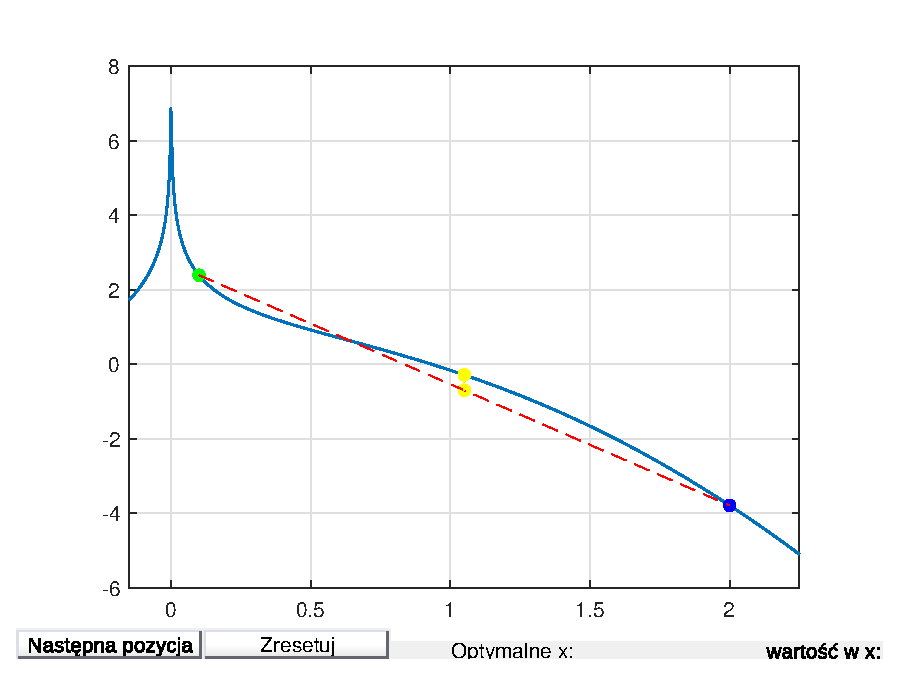
\includegraphics[width=\linewidth]{img/Bisection.eps}
        \caption{Początkowy stan przy dla funkcji drugiej}
            \label{fig:my_label}
        \end{figure}
        \par
        \null \vfill
        Można zaobserwować iż zielony punkt wyznacza $x_A$ a niebieski $x_B$. Metoda bisekcji polega na wyznaczaniu punktu po środku wyznaczanych punktów. W wyrysowanym przypadku widać iż punkt ten jest dokładnie na środku wyaproksymowanej prostej. 
        \vfill \null
    \end{multicols}
\end{figure}
\begin{figure}[H]
    \begin{multicols}{2}
        \null \vfill
        W przejściu iteracyjnym w miejsce wyznaczonego punktu środkowego, jeden z wcześniej orkeślonych punktów (W tym przypadku $x_B$) zostaje przeniesiony. Funkcja ponownie się wywołuje i wyznacza kolejny punkt środkowy między punktami.
        \vfill \null
        \par
        \begin{figure}[H]
            \centering
            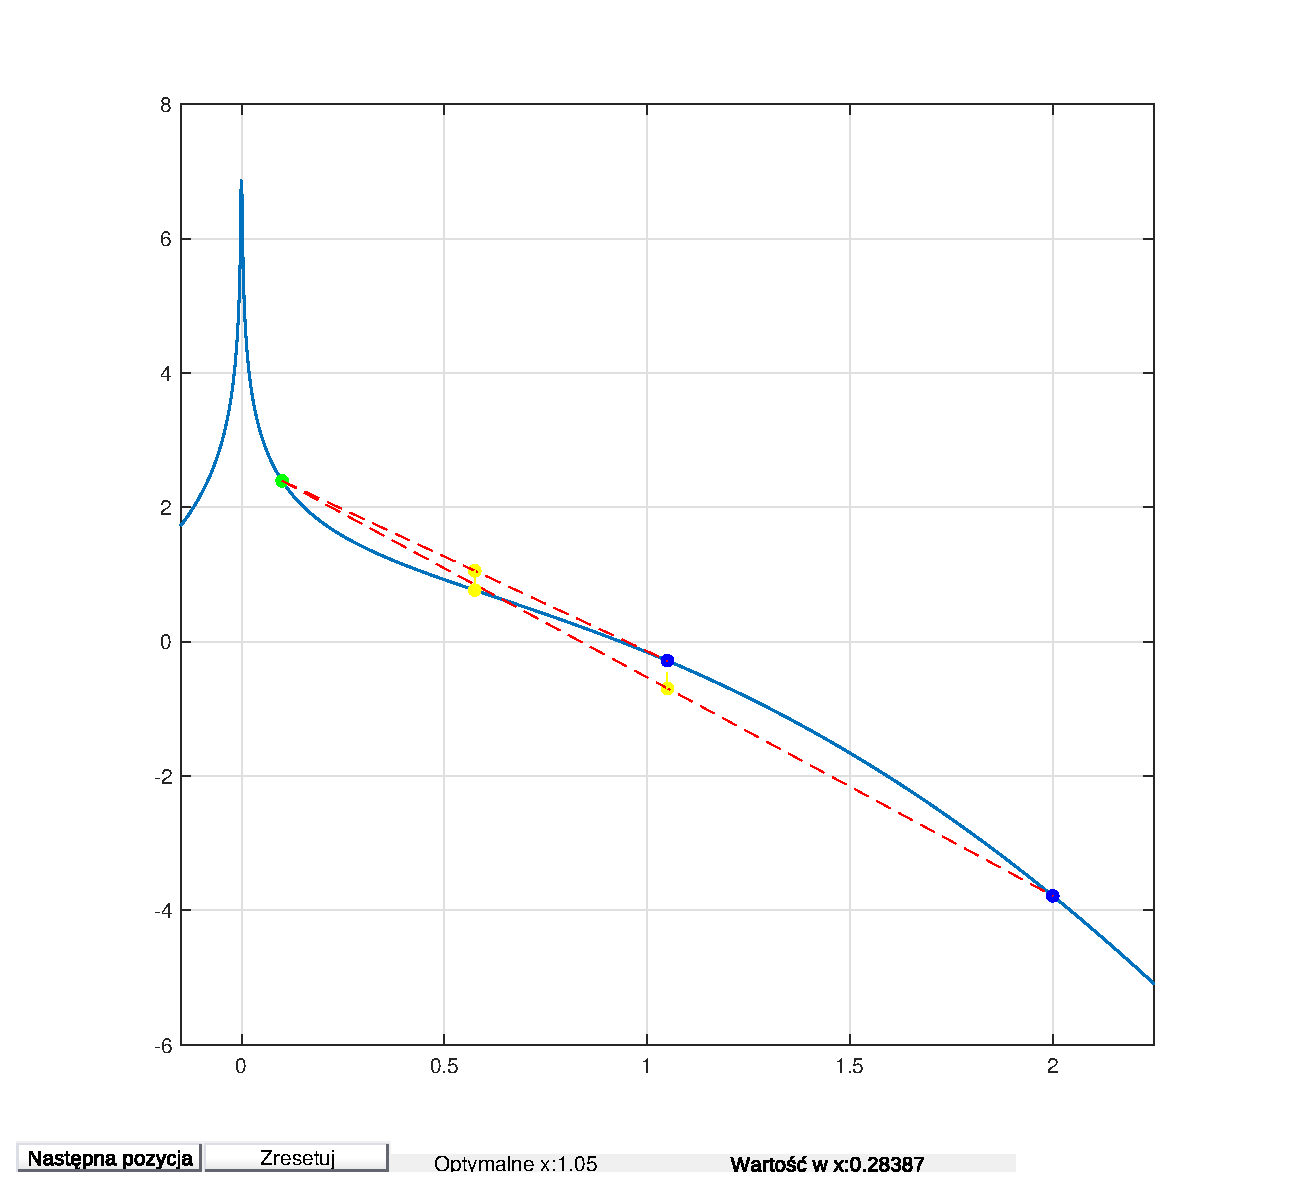
\includegraphics[width=\linewidth]{img/Bisection1.eps}
        \caption{Kolejna iteracja}
            \label{fig:my_label}
        \end{figure}
    \end{multicols}
\end{figure}
 Wykonywanie funkcji kończy się w momencie osiągnięcia rządanej precyzji bądź też po przekroczeniu ograniczenia iteracji wywołań funkcji.
\subsection{Metoda Iteracyjna: Regula Falsi}
Fałszywa krzywa jest metodą dość zbliżoną działaniem do wcześniej wykorzystanej metody bisekcji, natomiast tutaj korzystamy z własności "fałszywej prostej". Do wizualizacji posłużono się pierwszym przykładem.
\begin{figure}[H]
    \begin{multicols}{2}
        \null \vfill
        Metoda zaczyna się w podobny sposób do metody bisekcji. W celach wizualizacyjnych zakreślono odcinek między punktami $x_A$ i $x_B$. Wyznaczamy nowy potencjalny punkt skoku żółtymi kropkami, określony jest on przez przekroczenie wyinterpolowanego odcinka osi X. Pozycja nowego punktu na osi X wynosi $~1.1306$. Nowe współrzędne X, można oszacować danym równaniem $x_r = \frac{x_B*f(x_A) - x_A * f(x_B)}{f(x_A)-f(x_B)}$ 
        
        \vfill \null
        \par
        \begin{figure}[H]
            \centering
            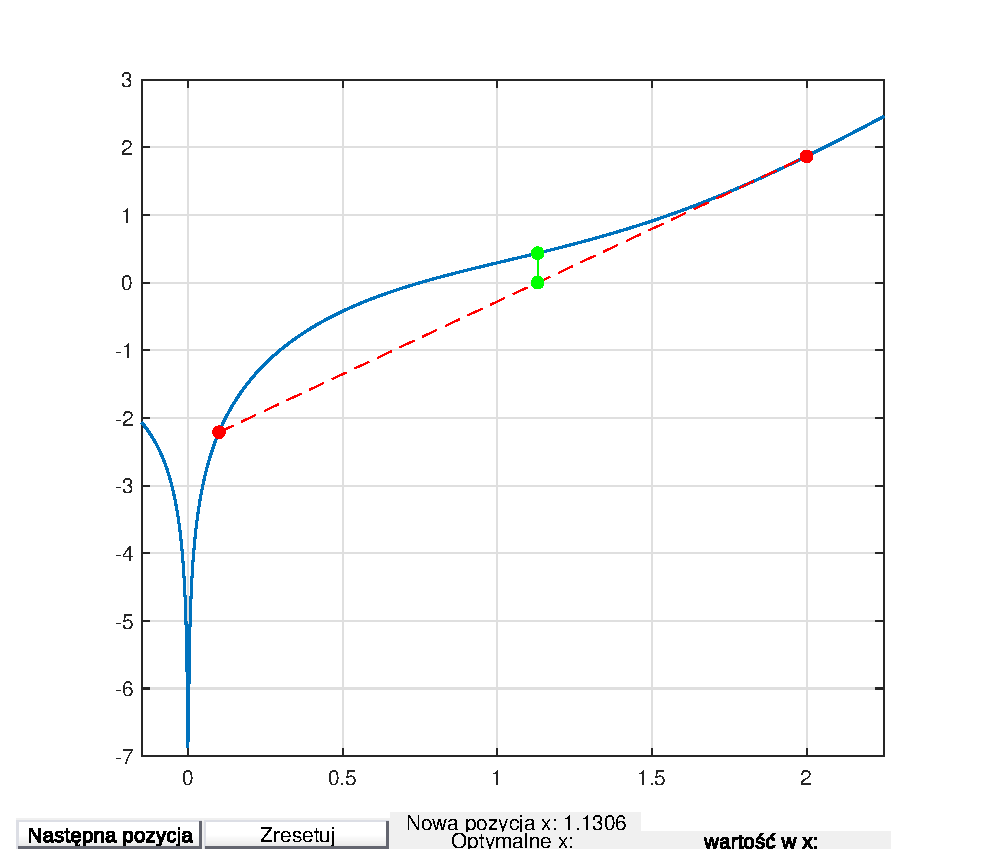
\includegraphics[width=\linewidth]{img/falsi.eps}
        \caption{Kolejna iteracja}
            \label{fig:my_label}
        \end{figure}
    \end{multicols}
\end{figure}
\begin{figure}[H]
    \begin{multicols}{2}
        \begin{figure}[H]
            \centering
            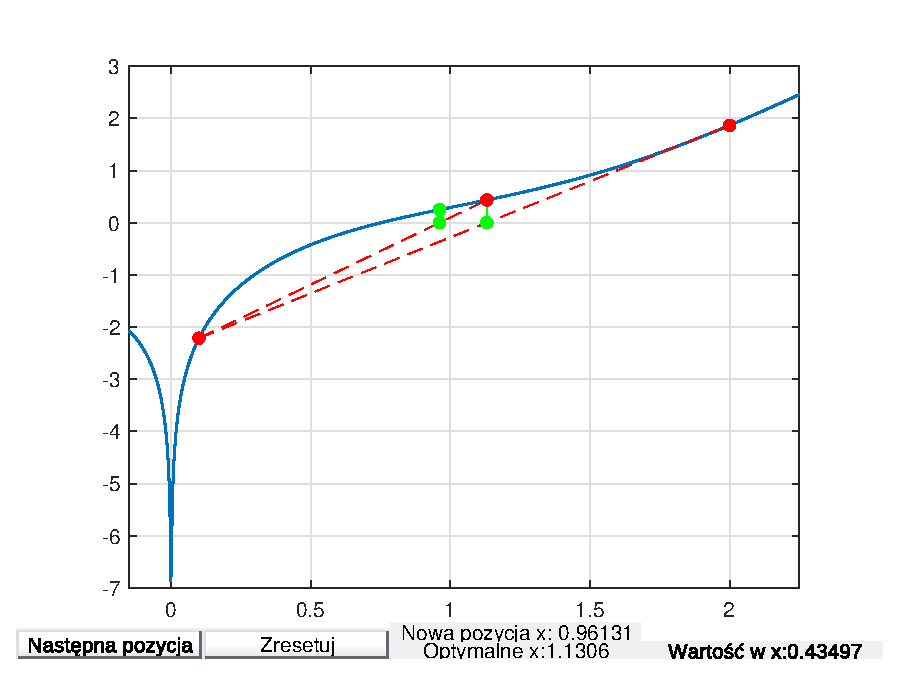
\includegraphics[width=\linewidth]{img/falsi1.eps}
        \caption{Kolejna iteracja}
            \label{fig:my_label}
        \end{figure}
        \par
        \null \vfill
        Nowo wyznaczony punkt posiadał dodatnią wartość funkcji ($f(1.1306) \approx 0.43497$), przez co zastąpił on punkt określający dodatnią wartość jakim był $x_B$. Powtarza się algorytm wyznaczający punkt przecięcia
        \vfill \null
    \end{multicols}
\end{figure}
\subsubsection{Uzyskane wyniki}
W obu przypadkach dla początkowych punktów w $x_A = 0.1$ i $x_B = 2$ oraz $tolFcn = 1e-4$.
\begin{itemize}
    \item Funkcja pierwsza $-sin^2  + x + log(x)$: $0.7517$
    \item Funkcja druga $sin(x) - x^2 - log(x)$: $0.9340$.
\end{itemize}
\section{Github, bibliografia, dokumentacja}
\begin{itemize}
    \item \url{https://github.com/Myknakryu/pok-2023}
    \item \url{https://traf-barak.pwr.edu.pl/wp-content/uploads/2020/08/Raport.pdf}
    \item \url{https://www.youtube.com/watch?v=xOLJMKGNivU}
\end{itemize}
\end{document}
